\documentclass[letterpaper,12pt,fleqn]{article}
\usepackage{matharticle}
\pagestyle{empty}
\newcommand{\A}{\mathcal{A}}
\renewcommand{\P}{\mathcal{P}}
\newcommand{\T}{\mathcal{T}}
\begin{document}
\section*{Topology}

\begin{definition}[Topology]
  A \emph{topology} $\T$ on a set $X$ is a subset of $\P(X)$ such that:
  \begin{enumerate}
  \item $\emptyset,X\in\T$
  \item $\T$ is closed under the operation of \emph{arbitrary} union.
  \item $\T$ is closed under the operation of \emph{finite} intersection.
  \end{enumerate}
  The ordered pair $(X,\T)$ is called a \emph{topological space}.
\end{definition}

\begin{definition}[Open]
  Let $(X,\T)$ be a topological space:
  \begin{itemize}
  \item To say that $U\subset X$ is an \emph{open set} means $U\in\T$.
  \item To say that $U\subset X$ is a \emph{closed set} means $X-U\in\T$.
  \end{itemize}
\end{definition}

\begin{example}
  Let $X=\{1,2,3\}$:

  \begin{minipage}{3in}
    \centering
    \begin{tikzpicture}
      \node at (0,1.25) {$1$};
      \node at (2,1.25) {$2$};
      \node at (1,-0.25) {$3$};
      \draw (1,0.75) circle [radius=2];
    \end{tikzpicture}
  \end{minipage}
  \begin{minipage}{3in}
    This is a topology on $X$.
  \end{minipage}

  \begin{minipage}{3in}
    \centering
    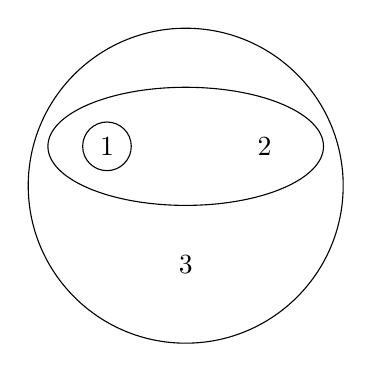
\begin{tikzpicture}
      \node [draw,circle] at (0,1.25) {$1$};
      \node at (2,1.25) {$2$};
      \node at (1,-0.25) {$3$};
      \draw (1,0.75) circle [radius=2];
      \draw (1,1.25) ellipse (1.75 and 0.75);
    \end{tikzpicture}
  \end{minipage}
  \begin{minipage}{3in}
    This is a topology on $X$.
  \end{minipage}

  \begin{minipage}{3in}
    \centering
    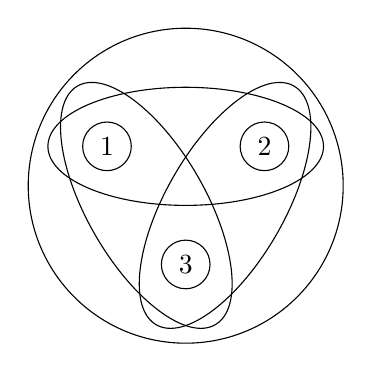
\begin{tikzpicture}
      \node [draw,circle] at (0,1.25) {$1$};
      \node [draw,circle] at (2,1.25) {$2$};
      \node [draw,circle] at (1,-0.25) {$3$};
      \draw (1,0.75) circle [radius=2];
      \draw (1,1.25) ellipse (1.75 and 0.75);
      \draw [rotate around={60:(1.5,0.5)}] (1.5,0.5) ellipse (1.75 and 0.75);
      \draw [rotate around={120:(0.5,0.5)}] (0.5,0.5) ellipse (1.75 and 0.75);
    \end{tikzpicture}
  \end{minipage}
  \begin{minipage}{3in}
    This is a topology on $X$.
  \end{minipage}

  \begin{minipage}{3in}
    \centering
    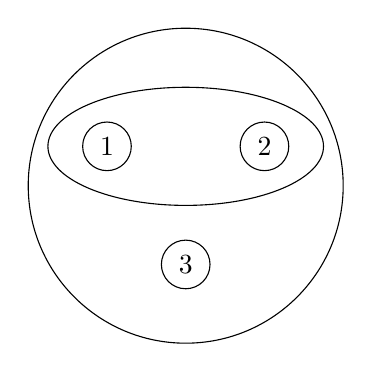
\begin{tikzpicture}
      \node [draw,circle] at (0,1.25) {$1$};
      \node [draw,circle] at (2,1.25) {$2$};
      \node [draw,circle] at (1,-0.25) {$3$};
      \draw (1,0.75) circle [radius=2];
      \draw (1,1.25) ellipse (1.75 and 0.75);
    \end{tikzpicture}
  \end{minipage}
  \begin{minipage}{4in}
    This is \emph{not} a topology on $X$ because $\{1\},\{3\}\in\T$; however
    $\{1\}\cup\{3\}=\{1,3\}\notin\T$.
  \end{minipage}
\end{example}

\begin{definition}[Discrete]
  Let $(x,\T)$ be a topological space:
  \begin{itemize}
  \item $\T=\{\emptyset,x\}$ is called the \emph{trivial} or \emph{indiscrete}
    topology.
  \item $\T=\P(X)$ is called the \emph{discrete} topology.
  \end{itemize}
\end{definition}

\begin{theorem}
  Let $X$ be a set. The discrete topology $\T$ on $X$ is a topology.
\end{theorem}

\begin{theproof}
  \listbreak
  \begin{enumerate}
  \item $\emptyset,X\subset X$ \\
    $\therefore\emptyset,X\in\P(X)=\T$

  \item Assume $\A\subset\P(X)$. \\
    Let $S=\bigcup_{A\in\A}A$. \\
    $S\subset X$ \\
    $\therefore S\in\P(X)=\T$

  \item Assume $\A=\left\{A_i\mid i\in\{1,\ldots,n\}\right\}\subset\P(X)$. \\
    Let $T=\bigcap_{i=1}^nA_i$. \\
    $T\subset X$ \\
    $\therefore T\in\P(X)=\T$
  \end{enumerate}
  $\therefore\T$ is a topology on $X$.
\end{theproof}

\end{document}
